% ************************************
\section{Quantum Speed-Ups}
% ************************************


\begin{frame}{The Quantum Speed-Ups}
 \begin{block}{Calculating the input of the Oracle:}
  Estimate $\Tr(Ap)$ for a hermitian matrix $A$ and a density operator $p$.
 \end{block}
 
 \begin{block}{A fast implementation of the Oracle:}
  Find a feasible solution of a linear programm.
 \end{block}
\end{frame}

\subsection{The input of the Oracle:}

\begin{frame}{First Speed-Up: Input of the Oracle}
 \begin{block}{Problem:}
  \textbf{Input:} Hermitian matrices $A,H$ \\
  \textbf{Output:} Approximation of $\Tr(Ap)$ with $p=\frac{e^{-H}}{\Tr(e^{-H})}$
 \end{block}
 
 \begin{block}{Note:}
  The output is not binary, but the probability of a qubit being $0$.\\
  \alert{$\Rightarrow$ We need to construct a quantum circuit, which turns a specific register (e.g. $\ket{0\ldots 0}$) into one where the first qubit is as needed.}
 \end{block} 
\end{frame}

\begin{frame}{The input of the Oracle: Linear programming}
\begin{block}{LP as a special case of SDP}
All matrices are diagonal matrices.
\alert{Calculation of $\Tr(Ap)$ becomes much easier!}
\end{block}

TODO calculate classically -> transform into probability

\end{frame}

\begin{frame}{The input of the Oracle: SDP}
TODO implement "functions of hamiltonians" for hermitian $H$: $f(H)=f(U Diag(\lambda_i) U^T)=U Diag(\tilde{f}(\lambda_i))U^T$

Use this to calc $\sqrt{H}$, $e^{-H}$
\end{frame}

\subsection{The Oracle}

%TODO Layout
\begin{frame}{The Oracle: Problem definition}
\textbf{Input: }
\begin{align*}
\alpha&\in\R\\
r&\in \R_{\geq 0}\\
a&\in \R^m \text{ with } a_j\approx \Tr(A_j p)\\
b&\in \R^m\\
c&\approx \Tr(Cp)-\varepsilon
\end{align*}
\textbf{Output: } $y\in \mathbb{R}^m$ with:
%TODO Fix spacing
% \begin{columns}
% \column{0.5\linewidth}
\begin{align*}
\|y\|_1&\leq r && \text{\structure{Compared to the dual SDP}}\\
b^T y&\leq \alpha&&\min \quad b^T y\\
a^T y&\geq c&&\text{s.t. } \quad \sum_{j=1}^m y_j A_j - C\succeq 0\\
y&\geq 0 && \qquad y\geq 0
\end{align*}
% \column{0.5\linewidth}
% \begin{block}{Compared to the dual SDP:}
% \begin{align*}
% \min\quad&b^T y\\
% \text{s.t. }&\sum_{j=1}^m y_j A_j - C\succeq 0\\
% &y\geq 0
% \end{align*}
% \end{block}

% \end{columns}
\end{frame}

\begin{frame}{Simplifying the problem}
Substituting $y=Nq$ with $N=\|y\|_1$ and $\|q\|_1=1$ results in:

%Some ugly magic for rcases inside of align
\begin{equation*}
 \begin{split}
  b^T q&\leq \alpha/N\\
  a^T q&\geq c/N\\
  \begin{aligned}
   \|q\|_1\\
   q
  \end{aligned}
  &
  \begin{rcases*}
   =1\\
   \geq 0
  \end{rcases*} \text{convex combination coefficients}  \\
  0&<N\leq r
 \end{split}
\end{equation*}
\end{frame}

\begin{frame}{Simplifying the problem}
\begin{block}{Problem: two-dimensional interpretation}
Find the convex combination of a point $P\in\mathrm{conv}\{p_i=(b_i,a_i)\}$,\\
which lies to the upper left of $(\alpha/N, c/N)$ for an $0<N\leq r$.
\end{block}

\vspace{1cm}

Define $G_N$ as the upper-left quadrant starting at $(\alpha/N, c/N)$.
Define $G$ as the union of all $G_N$ with $0<N\leq r$.

\end{frame}

\begin{frame}{Understanding the area $G$}


\begin{columns}
\column{0.36\linewidth}

\raggedleft
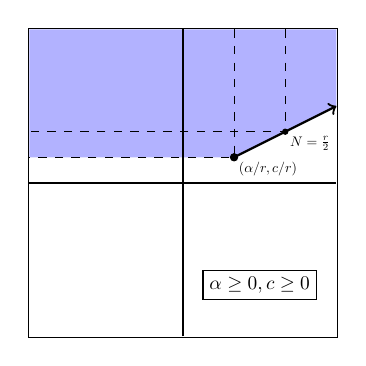
\begin{tikzpicture}[scale=0.65]%[shift={(11cm,-1.5cm)}]
\contourlength{0.5mm};

\coordinate[label={[scale=0.5]below right: {$(\alpha/r,c/r)$}}] (ac) at (1,1/2);
\coordinate[label={[scale=0.5]below right: {$N=\frac{r}{2}$}}]  (ac2) at (2,1);
\coordinate													    (ac3) at (3,3/2);

\fill[blue!30!white] (ac)--(ac -| -3,0)--(-3,3)--(ac3 |- 0,3)--(ac3)--cycle;

\draw[thick] (-3,0)--(3,0);
\draw[thick] (0, -3)--(0,3);
\draw[dashed] (ac |- 0,3) -- (ac) -- (ac -| -3,0);
\draw[dashed] (ac2 |- 0,3) -- (ac2) -- (ac2 -| -3,0);

\filldraw (ac) circle(0.07);
\filldraw (ac2) circle(0.05);

\draw[->, thick] (ac)--(ac3);

\node[scale=0.7,draw] at (1.5,-2) {$\alpha\geq 0, c\geq 0$};
\draw (current bounding box.north east) rectangle (current bounding box.south west);
\end{tikzpicture}


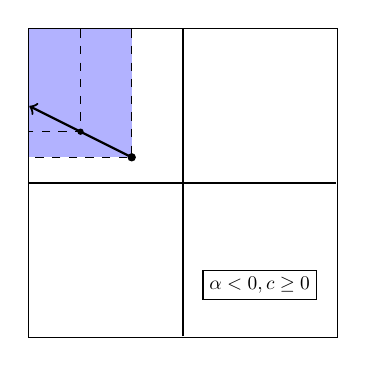
\begin{tikzpicture}[scale=0.65]%[shift={(11cm,-1.5cm)}]
\contourlength{0.5mm};

\coordinate (ac) at (-1,1/2);
\coordinate (ac2) at (-2,1);
\coordinate	(ac3) at (-3,3/2);

\fill[blue!30!white] (ac)--(ac -| -3,0)--(-3,3)--(ac |- 0,3)--cycle;

\draw[thick] (-3,0)--(3,0);
\draw[thick] (0, -3)--(0,3);
\draw[dashed] (ac |- 0,3) -- (ac) -- (ac -| -3,0);
\draw[dashed] (ac2 |- 0,3) -- (ac2) -- (ac2 -| -3,0);

\filldraw (ac) circle(0.07);
\filldraw (ac2) circle(0.05);

\draw[->, thick] (ac)--(ac3);

\node[scale=0.7,draw] at (1.5,-2) {$\alpha < 0, c\geq 0$};
\draw (current bounding box.north east) rectangle (current bounding box.south west);
\end{tikzpicture}
\column{0.36\linewidth}

\raggedright
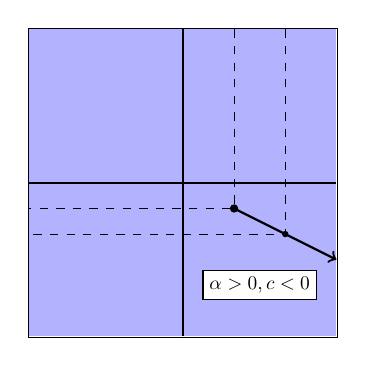
\begin{tikzpicture}[scale=0.65]%[shift={(11cm,-1.5cm)}]
\contourlength{0.5mm};

\coordinate (ac) at (1,-1/2);
\coordinate (ac2) at (2,-1);
\coordinate	(ac3) at (3,-3/2);

\fill[blue!30!white] (-3,-3)--(-3,3)--(3,3)--(3,-3)--cycle;

\draw[thick] (-3,0)--(3,0);
\draw[thick] (0, -3)--(0,3);
\draw[dashed] (ac |- 0,3) -- (ac) -- (ac -| -3,0);
\draw[dashed] (ac2 |- 0,3) -- (ac2) -- (ac2 -| -3,0);

\filldraw (ac) circle(0.07);
\filldraw (ac2) circle(0.05);

\draw[->, thick] (ac)--(ac3);

\node[scale=0.7,draw, fill=white] at (1.5,-2) {$\alpha > 0, c < 0$};
\draw (current bounding box.north east) rectangle (current bounding box.south west);
\end{tikzpicture}


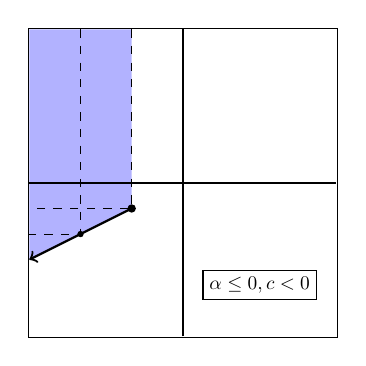
\begin{tikzpicture}[scale=0.65]%[shift={(11cm,-1.5cm)}]
\contourlength{0.5mm};

\coordinate (ac) at (-1,-1/2);
\coordinate (ac2) at (-2,-1);
\coordinate	(ac3) at (-3,-3/2);

\fill[blue!30!white] (ac)--(ac |- -3,3)--(-3,3)--(ac3)--cycle;

\draw[thick] (-3,0)--(3,0);
\draw[thick] (0, -3)--(0,3);
\draw[dashed] (ac |- 0,3) -- (ac) -- (ac -| -3,0);
\draw[dashed] (ac2 |- 0,3) -- (ac2) -- (ac2 -| -3,0);

\filldraw (ac) circle(0.07);
\filldraw (ac2) circle(0.05);

\draw[->, thick] (ac)--(ac3);

\node[scale=0.7,draw] at (1.5,-2) {$\alpha \leq 0, c < 0$};
\draw (current bounding box.north east) rectangle (current bounding box.south west);
\end{tikzpicture}

\column{.28\textwidth}
If $\alpha > 0, c < 0$, then is $G=\R^2$. 

\vspace{1cm}
Otherwise $G$ is the intersection of two half-planes.

\end{columns}

\end{frame}

\begin{frame}{2-sparse solutions}
\begin{tikzpicture}
\contourlength{0.5mm};
\shade[lower right=blue!60!white] (0,0) rectangle (3,3);
\node at (1,2) {\contour{white}{$G_N$}};
\filldraw[thick, fill=red!20!white, fill opacity=0.3] (0,-1)--(4,3)--(6,2)--(4,-2)--(2,-2)--cycle;
\draw[red, thick] (1,0)--(3,2);
\node[anchor=south] at (4,3) {$Q=\mathrm{conv}\{p_i|1\leq i \leq m\}$};
\draw (0,-1)--(6,2)--(2,-2)--(4,3)--(4,-2)--cycle;
\filldraw (2.5,0.5) circle(0.07) node[anchor=south east]{\contour{white}{$P$}};
\filldraw (3,0) circle(0.07) node[anchor=north west]{\contour{white}{$(\alpha/N,c/N)$}};
\node[text width=5cm] at (9,0) 
	{If there is no $p_i\in G_N$\\
	but there is a $P\in G_N\cap Q$\\
	then $\partial Q\cap G_N\neq \emptyset$.\\ 
	\vspace{0.5cm}
	In particular, there is a line with $\overline{p_i p_j}\cap G_N\neq\emptyset$.\\
	\vspace{0.5cm}
	That means we can always find a 2-sparse solution $q$.};
\end{tikzpicture}
\end{frame}



\begin{frame}{The algorithm}
\begin{algorithmic}
\If{$\alpha\geq 0$ and $c\leq 0$}
	\Comment{Check if $G=\R^2$}
    \State \Return $y=0$
    \pause
\ElsIf{$\exists i: p_i\in G$}
	\Comment{Check if a corner is in $G$}
    \State \Return $y=Ne_i$ with $N=c/a_i$
    \pause
\Else
	\Comment{Search a 2-sparse solution}
	\State Find $j,k$ such that $\overline{p_j p_k}\cap G\neq \emptyset$
	\If{Such $j,k$ exist}
		\State Calculate a fitting convex combination $q$ and scalar $N$
		\State \Return $y=Nq$
	\Else
		\State \Return	No $y$ found.
	\EndIf
\EndIf
\end{algorithmic}
\end{frame}

\begin{frame}{How to find $j,k$ with $\overline{p_j p_k}\cap G\neq \emptyset$}
\begin{tikzpicture}
\contourlength{0.5mm};
\coordinate[label=below left:$L_1$] (L1) at (0,0);
\coordinate[label=above right:$L_2$] (L2) at (3,3);
\coordinate[label=below right:{$(\alpha/r,c/r)$}] (g) at (3,0);
\coordinate[label=below left:$p_j$] (pj) at (1,-1);
\coordinate[label=above right:$p_k$] (pk) at (4,2);

\shade[lower right=blue!60!white] (L1) rectangle (3,3);
\draw[thick] (g)--(L1);
\draw[thick] (g)--(L2);
\node at (1,2) {\contour{white}{$G$}};
\filldraw (g) circle(0.05);
\filldraw (pj) circle(0.05);
\filldraw (pk) circle(0.05);
\draw (g)--(pj);
\draw (g)--(pk);
\draw[dashed] (pj)--(pk);

\begin{scope}
\path[clip] (g) -- (pj) -- (L1);
\draw (g) circle (0.8);
\end{scope}
%\node[scale=0.5] at (2.3,-0.1)  {$\sphericalangle p_j L_1$};

\begin{scope}
\path[clip] (g) -- (L1) -- (L2);
\draw (g) circle (0.6);
\end{scope}
%\node[scale=0.5] at (2.6,0.2) {$\sphericalangle L_1 L_2$};

\begin{scope}
\path[clip] (g) -- (L2) -- (pk);
\draw (g) circle (0.8);
\end{scope}
%\node[scale=0.5] at (3.2,0.9) {$\sphericalangle L_2 p_k$};

\node[text width=5.5cm] at (8,1) 
	{The angle $\sphericalangle L_1 L_2$ is constant.\\
	\vspace{0.5cm}
	The line $\overline{p_j p_k}$ crosses $G$ if and only if\\
	$\sphericalangle p_j L_1+\sphericalangle L_1 L_2
	    +\sphericalangle L_2 p_k\leq \pi$\\
	\vspace{0.5cm}
	\alert{$\Rightarrow$ Minimize $\sphericalangle p_j L_1$ and 
		$\sphericalangle L_2 p_k$   seperately!}};
\end{tikzpicture}
\end{frame}

\begin{frame}{Where is the quantum speed-up?}
\begin{block}{Step 2: Check if there is a $p_i\in G$}
If we implement the function $i\to$"Is $p_i\in G$?" as a quantum circuit, then Grover search can be used to find such a $p_i$ in $\mathcal{O}(\sqrt{m})$.
\end{block}

\begin{block}{Step 3: Minimize the angles $\sphericalangle p_j L_1$ and 
		$\sphericalangle L_2 p_k$}
If we implement the functions $i\to\sphericalangle p_i L_1$ and $i\to \sphericalangle L_2 p_k$ as quantum circuits, then the quantum minimum-finding algorithm of Dürr and Høyer can be used to minimize them in $\mathcal{O}(\sqrt{m})$.
\end{block}
\end{frame}

%Chapter 4?
\subsection{Runtime of the SDP solver}

\subsection{Downsides}

\subsection{Conclusions}